\tikzstyle{end} = [thin, circle, minimum size = 0.1cm, draw, inner sep = 0.1pt]
\tikzstyle{leaf} = [thin, circle, minimum size = 0.6cm, draw, inner sep = 0.1pt, blue]
\tikzstyle{inner} = [thin, circle, minimum size = 0.2cm, draw, inner sep = 0.1pt, black]
            


\tikzstyle{ed} = [thick, ->, draw, black]

    
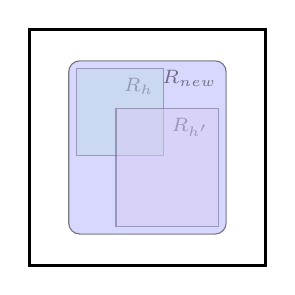
\begin{tikzpicture}[black]
    \draw[very thick] (0, 0) rectangle (3, 3);
    
    \draw[fill = green!20!white, opacity = 0.5] (0.6, 1.4) rectangle (1.7, 2.5) node[below left] {\scriptsize $R_{h}$};
    \draw[fill = red!10!white, opacity = 0.5] (1.1, 0.5) rectangle (2.4, 2.0) node[below left] {\scriptsize $R_{h'}$};

    \only<7->{
    	\draw[fill = blue!30!white, opacity = 0.5, rounded corners] (0.5, 0.4) rectangle (2.5, 2.6) node[below left]
	        {\scriptsize $R_{new}$};
    }
\end{tikzpicture}
